\chapter{ペトリネットに基づく変換前の多目的量子最適化}
\label{chap:poordirection}
量子インスパイアード最適化の論文\cite{shinjo}の定式化を参考にMRFSSPの各タスクのリソースコストとタスク間の待機時間の最適化を図る検証を行った.
\section{多資源フローショップスケジューリング問題}

\subsection{ペトリネットモデル}

\begin{figure}[H]
    \centering
    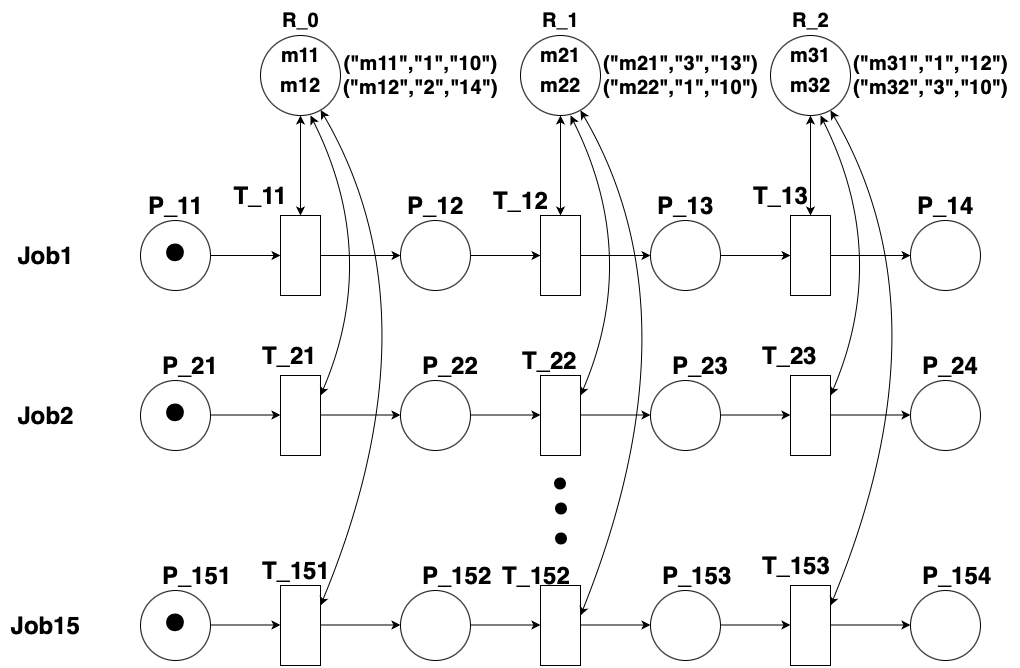
\includegraphics[width=0.8\linewidth, height=8cm]{./images/fsp.png}
    \caption{フローショップシステムのペトリネットモデル}
    \label{fig:fig1}
\end{figure}

MRFSSPに対するペトリネットモデルは,図\ref{fig:fig1}のように表現できる.図\ref{fig:fig1}では,15個のジョブを省略した形で記載している.各ジョブはプレース,トランジションの交互列となるパスで表されている.例えば,Job1に対するパス$P_{1,1}, T_{1,1}, P_{1,2}, ..., P_{1,4}$は,3種類のタスク(工程)$T_{1,1}, T_{1,2}, T_{1,3}$から構成されており,それぞれ,$R_0, R_1, R_2$のマシンリソースを必要としている.3種類のマシンリソースは,カラートークンとしてマシンID,処理速度,マシンコストの情報を含む文字列で表されている.このシステムの目的は,ペトリネットにおける繊維が順序通りに発火することにより最終的に全てのトークンがモデルの最右端に到達することである.これはスケジューリングの完了を意味する.この過程においては,システムに課された全ての制約が満たされることが前提となり,加えて目的関数の最適化が達成されることが重要である.すなわち,最適化されたスケジューリングにおいては,リソースの利用効率や処理時間などの複数の要素がバランスよく最適化される必要がある.このペトリネットモデルのようにドメイン知識さえあれば,わずかなペトリネットの記述のルールに基づいてペトリネットモデルを作成することができる.

\subsection{CPNToolsによるモデル生成}
CPNToolsは,カラードペトリネットのモデリングおよびシミュレーションを支援するツールである.本研究では,CPNToolsを用いて生成したペトリネットモデルをXML形式でエクスポートすることで,プレース,アーク,トランジションに関する構造情報および動作情報を取得する.

プレース,トランジション,アークのXMLファイルの一部を以下に示す.

\lstset{
  basicstyle={\ttfamily},
  identifierstyle={\small},
  commentstyle={\smallitshape},
  keywordstyle={\small\bfseries},
  ndkeywordstyle={\small},
  stringstyle={\small\ttfamily},
  frame={tb},
  breaklines=true,
  columns=[l]{fullflexible},
  numbers=left,
  xrightmargin=0zw,
  xleftmargin=3zw,
  numberstyle={\scriptsize},
  stepnumber=1,
  numbersep=1zw,
  lineskip=-0.5ex
}
\begin{lstlisting}[caption=プレースのXMLファイル,label=cpn_place]
<place id="ID1412324394">
        <posattr x="-284.000000"
                 y="42.000000"/>
        <fillattr colour="White"
                  pattern=""
                  filled="false"/>
        <lineattr colour="Black"
                  thick="1"
                  type="Solid"/>
        <textattr colour="Black"
                  bold="false"/>
        <text>p_11</text>
        <ellipse w="60.000000"
                 h="40.000000"/>
        <token x="-10.000000"
               y="0.000000"/>
        <marking x="0.000000"
                 y="0.000000"
                 hidden="false">
          <snap snap_id="0"
                anchor.horizontal="0"
                anchor.vertical="0"/>
        </marking>
        <type id="ID1412324395">
          <posattr x="-244.000000"
                   y="18.000000"/>
          <fillattr colour="White"
                    pattern="Solid"
                    filled="false"/>
          <lineattr colour="Black"
                    thick="0"
                    type="Solid"/>
          <textattr colour="Black"
                    bold="false"/>
          <text tool="CPN Tools"
                version="4.0.1">UNIT</text>
        </type>
        <initmark id="ID1412324396">
          <posattr x="-255.000000"
                   y="65.000000"/>
          <fillattr colour="White"
                    pattern="Solid"
                    filled="false"/>
          <lineattr colour="Black"
                    thick="0"
                    type="Solid"/>
          <textattr colour="Black"
                    bold="false"/>
          <text tool="CPN Tools"
                version="4.0.1">1`()</text>
        </initmark>
      </place>
\end{lstlisting}

Listing \ref{cpn_place}は,プレースに関する情報であり<place id>はアークとの関連付けに使用するためのユニークなIDである.<text>プレース</text>はプレースのラベルが指定されており人間が理解しやすい形になっている.<initmark id>はトークンのユニークなIDであり<text tool>トークンの数‘()</text>で初期状態でのトークンの数を表している.

\begin{lstlisting}[caption=トランジションのXMLファイル,label=cpn_transition]
<trans id="ID1412324537"
             explicit="false">
        <posattr x="-138.000000"
                 y="42.000000"/>
        <fillattr colour="White"
                  pattern=""
                  filled="false"/>
        <lineattr colour="Black"
                  thick="1"
                  type="solid"/>
        <textattr colour="Black"
                  bold="false"/>
        <text>t_11</text>
        <box w="60.000000"
             h="38.000000"/>
        <binding x="7.200000"
                 y="-3.000000"/>
        <cond id="ID1412324538">
          <posattr x="-177.000000"
                   y="72.000000"/>
          <fillattr colour="White"
                    pattern="Solid"
                    filled="false"/>
          <lineattr colour="Black"
                    thick="0"
                    type="Solid"/>
          <textattr colour="Black"
                    bold="false"/>
          <text tool="CPN Tools"
                version="4.0.1"/>
        </cond>
        <time id="ID1412324539">
          <posattr x="-93.500000"
                   y="72.000000"/>
          <fillattr colour="White"
                    pattern="Solid"
                    filled="false"/>
          <lineattr colour="Black"
                    thick="0"
                    type="Solid"/>
          <textattr colour="Black"
                    bold="false"/>
          <text tool="CPN Tools"
                version="4.0.1"/>
        </time>
        <code id="ID1412324540">
          <posattr x="-73.500000"
                   y="-9.000000"/>
          <fillattr colour="White"
                    pattern="Solid"
                    filled="false"/>
          <lineattr colour="Black"
                    thick="0"
                    type="Solid"/>
          <textattr colour="Black"
                    bold="false"/>
          <text tool="CPN Tools"
                version="4.0.1"/>
        </code>
        <priority id="ID1412324542">
          <posattr x="-206.000000"
                   y="12.000000"/>
          <fillattr colour="White"
                    pattern="Solid"
                    filled="false"/>
          <lineattr colour="Black"
                    thick="0"
                    type="Solid"/>
          <textattr colour="Black"
                    bold="false"/>
          <text tool="CPN Tools"
                version="4.0.1"/>
        </priority>
      </trans>
\end{lstlisting}

Listing \ref{cpn_transition}は,トランジションに関する情報でありプレース同様にプレースとアークの関連付けに使用するためのユニークなIDが付与されている.また,text要素にはトランジションのラベルが指定されている.さらに,<cond>はトランジションの発火条件,<priority>は発火の優先順位,<time>トランジションの処理時間を記載する要素である.ただし,本研究では<cond>,<priority>,および<time>には設定を行っていない.

\begin{lstlisting}[caption=アークのXMLファイル,label=cpn_arc]
<arc id="ID1412324579"
           orientation="PtoT"
           order="1">
        <posattr x="0.000000"
                 y="0.000000"/>
        <fillattr colour="White"
                  pattern=""
                  filled="false"/>
        <lineattr colour="Black"
                  thick="1"
                  type="Solid"/>
        <textattr colour="Black"
                  bold="false"/>
        <arrowattr headsize="1.200000"
                   currentcyckle="2"/>
        <transend idref="ID1412324537"/>
        <placeend idref="ID1412324394"/>
        <annot id="ID1422288249">
          <posattr x="-211.000000"
                   y="53.000000"/>
          <fillattr colour="White"
                    pattern="Solid"
                    filled="false"/>
          <lineattr colour="Black"
                    thick="0"
                    type="Solid"/>
          <textattr colour="Black"
                    bold="false"/>
          <text tool="CPN Tools"
                version="4.0.1">1`()</text>
        </annot>
      </arc>
\end{lstlisting}

Listing \ref{cpn_arc}は,アークに関する情報でありユニークなIDが付与されている.<arc orientation>では,アークの接続方向の指定がされている.PtoTはプレースからトランジション,TtoPはトランジションからプレースの接続を意味する.

上記のXMLファイルから得られた情報を表にまとめる.

\begin{table}[ht]
    \centering
    \caption{XMLファイルから取得した情報}
    \begin{tabular}{|c|p{0.6\linewidth}|} % 列の定義に縦線を追加
        \hline
        \textbf{リスト} & \textbf{取得情報} \\
        \hline
        \textit{resource\_m} & マシンリソースのラベルとリソースの複数の性能 \\
        \textit{machine\_processing\_time} & 単位時間あたりの処理時間 \\
        \textit{machine\_cost} & 単位時間あたりのコスト \\
        \textit{job} & 各ジョブのタスクを順番に並べた構造 \\
        \hline
    \end{tabular}
    \label{variable}
\end{table}


\subsection{QUBO定式化}
基本的なQUBO定式化の方式に基づいてMRFSSPのペトリネットモデルからの定式化を行う.これらの式で用いた変数を表\ref{variable}にまとめる.

\begin{table}[ht]
    \centering
    \caption{エネルギー関数内の変数}
    \begin{tabular}{>{$}c<{$} p{0.6\linewidth}}
        \hline
        \text{変数} & \text{定義} \\
        \hline
        rc^r & 単位時間あたりのマシンリソース$r$の使用コスト \\
        fd^r & マシンリソース$r$を使ってタスクを処理する場合の処理時間 \\
        t_{i}^{j} & ジョブ$j$の$i$番目のタスク \\
        x_{k}^{r}(t_{i}^{j}) & 時刻$k$において$t_{i}^{j}$がマシンリソース$r$を使用していれば$x_{k}^{r}(t_{i}^{j})=1$,そうでなければ$0$を示すバイナリ変数 \\
        \hline
    \end{tabular}
    \label{variable}
\end{table}

ペトリネットの発火規則に従うためには,以下のエネルギー関数をゼロにする必要がある.すなわち,$E_{c1}$及び$E_{c2}$ともトランジションズの発火にはその入力プレース全てにトークンが配置されている必要があり,かつ,同じ入力プレースで同じトークンを前提に発火を行うことは禁止されているため,その競合状態にある場合には,一つのトランジションの発火のみに当該トークンが利用される必要がある.このようにペトリネットの発火規則から以下のエネルギー関数が生成できる.

\begin{align} 
E_{c1} &= \sum_{k_1,k_2} \sum_r \sum_{(j_1,j_2)} \sum_i x_{k_1}^{r}(t_{i}^{j_1}) \cdot x_{k_2}^{r}(t_{i}^{j_2}) \label{eqn:c1}\\ 
E_{c2} &= \sum_{k_1,k_2} \sum_{r_1,r_2} \sum_j \sum_i x_{k_1}^{r_1}(t_{i}^{j}) \cdot x_{k_2}^{r_2}(t_{i+1}^{j}) \label{eqn:c2} 
\end{align}

一方,本スケジューリング問題は,全てのジョブが完了するまでタスクの実行計画を作成することであるので,全てのトランジションがただ一度ずつ発火する必要がある.これより,以下のエネルギー関数が生成できる.

\begin{align} 
E_{c3} &= \left( 1 - \sum_k \sum_r \sum_j \sum_i x_{k}^{r}(t_{i}^{j}) \right)^2 \label{eqn:c3} 
\end{align}

目的関数として,リソースの総コストの最小化とタスクの処理の待機時間の最小化となるため,ペトリネットの振る舞いモデルより以下のエネルギー関数が導かれる.

\begin{align} 
E_{o1} &= \sum_k \sum_r \sum_j \sum_i rc^r \cdot fd^r \cdot x_{k}^{r}(t_{i}^{j}) \label{eqn:o1}\\
E_{o2} &= \sum_i \sum_{k_1,k_2} \sum_{r_1,r_2} \sum_j \sum_i \left( k_1 - fd^{r_2} \right) \cdot x_{k_2}^{r_2}(t_{i+1}^{j}) \cdot x_{k_1}^{r_1}(t_{i}^{j}) \label{eqn:o2} 
\end{align}

式(\ref{eqn:c1}), (\ref{eqn:c2}), (\ref{eqn:c3}), (\ref{eqn:o1}), (\ref{eqn:o2})に重み$A$, $B$, $C$, $D$, $E$を乗じてまとめた全体のエネルギー関数は以下のようになる.

\begin{align} 
E = &A \cdot E_{c1} + B \cdot E_{c2} + C \cdot E_{c3} \ + D \cdot E_{o1} + E \cdot E_{o2} 
\end{align}

\section{評価実験}
ペトリネットモデルからQUBOモデルに定式化したエネルギー関数の最適化を行う.本実験では,OpenJij\cite{openjij}を用いて最適化計算を行う.問題設定は以下に示す.

\begin{enumerate} 
\item ジョブの数は5個. 
\item パラメータA,B,Cは制約の重み.
\item パラメータDはresource costの重み.
\item パラメータEはwaiting timeの重み.
\item 最適化計算をOpenJijで100回行いベイズ最適化でパラメータチューニングを行う.
\item 5. を5回繰り返す.
\end{enumerate}

\begin{figure}[H]
    \centering
    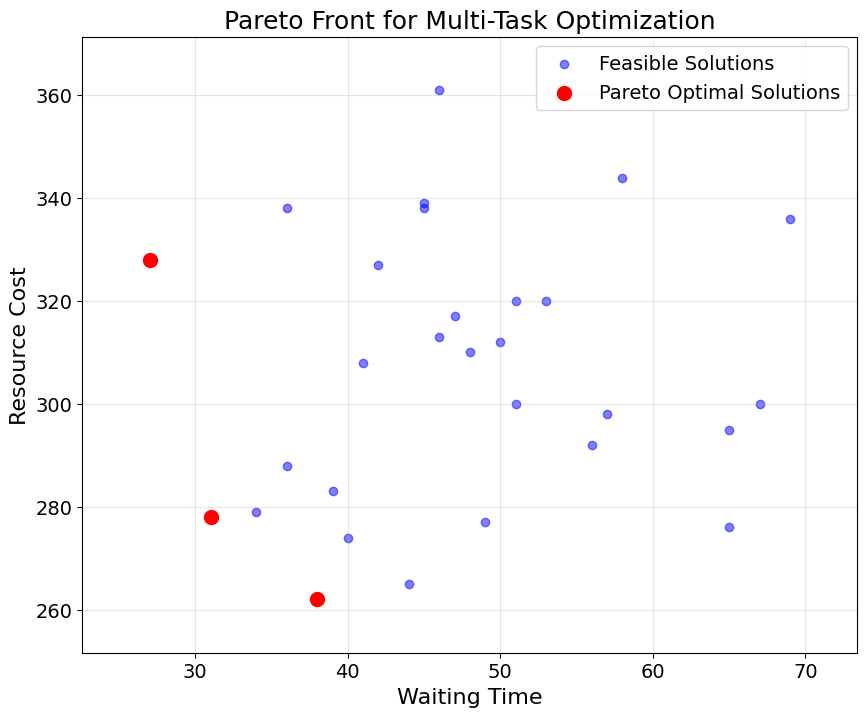
\includegraphics[width=0.8\linewidth, height=8cm]{./images/parato_job5.png}
    \caption{ペトリネット変換前のMRFSSPのパレート解}
    \label{fig:fig2}
\end{figure}

\begin{table}[ht]
    \centering
    \vspace{-0.3cm}
    \caption{各巡回における実行可能解と個数および平均値}
    \begin{tabular}{|c|c|c|c|}
        \hline
         巡回 & 個数 & Resource Costの平均値 & Waiting Timeの平均値 \\
        \hline
        第1巡 & 9 & 312.6 & 47 \\
        \hline
        第2巡 & 8 & 302.4 & 49.4 \\
        \hline
        第3巡 & 6 & 300 & 44.7\\
        \hline
        第4巡 & 2 & 328 & 55.5 \\
        \hline
        第5巡 & 4 & 297.5 & 44.8 \\
        \hline
        全体の平均 & 5.8 & 308.1 & 48.3 \\
        \hline
    \end{tabular}
    \label{tab:before_feasible}
\end{table}

表\ref{tab:before_feasible}は一度の最適化計算で得られた実行可能解の個数と,それらのResource CostおよびWaiting Timeの平均値を示している.平均値は実行可能解で得られた数で算出している.また,図\ref{fig:fig2}はペトリネット変換前のMRFSSPの最適化計算を行い,得られたパレート解を可視化したグラフになっている.

\begin{figure}[H]
    \centering
    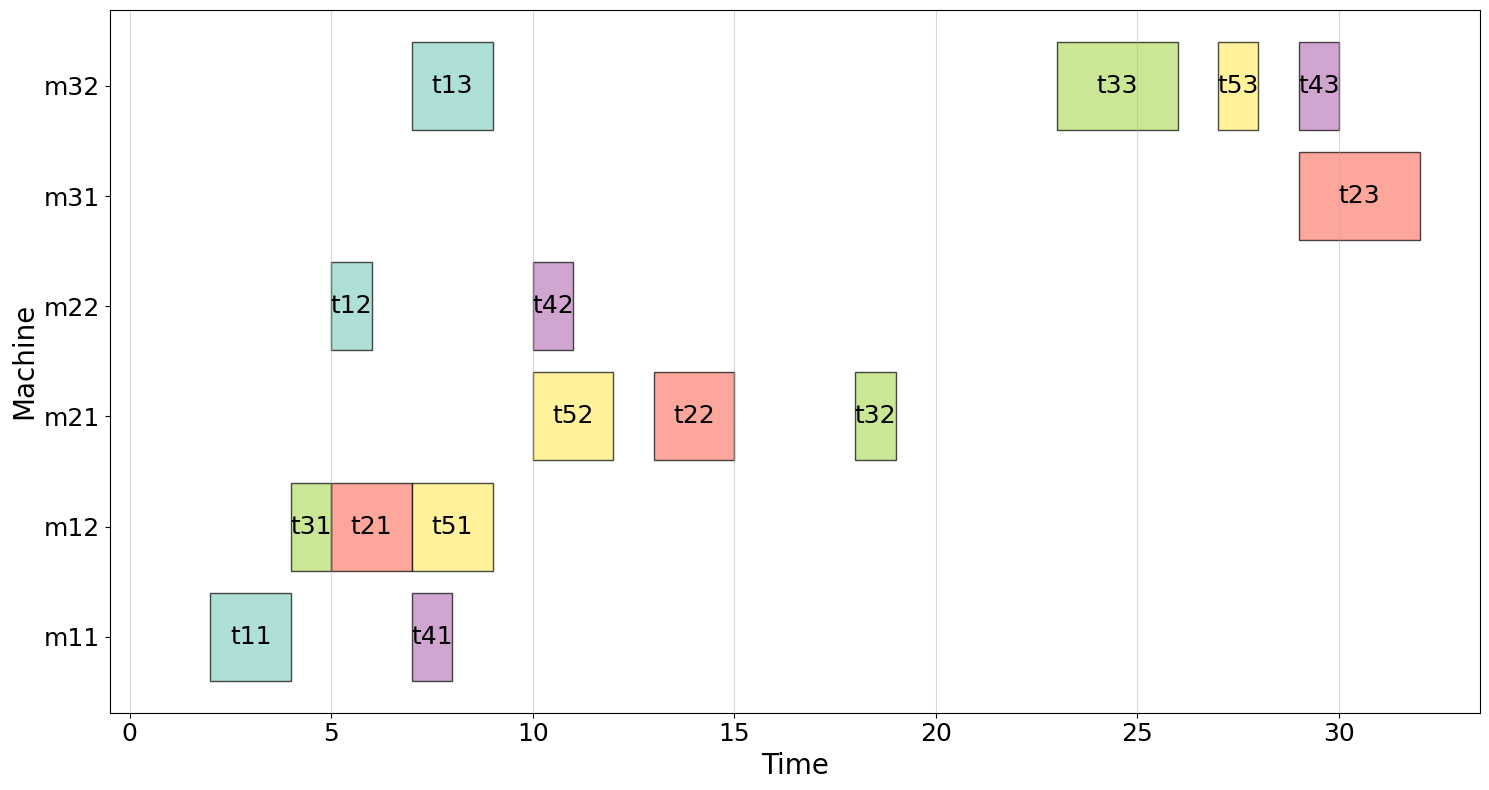
\includegraphics[width=0.8\linewidth, height=8cm]{./images/gantt1_job5.png}
    \caption{5個のジョブに対するスケジュール}
    \label{fig:fig3}
\end{figure}

図\ref{fig:fig3}は,計算結果の一例をガントチャートに表したものである.本ガントチャートでは,色分けによりジョブごとのタスクが区別されており,ジョブ全体の進行状況が視覚的に把握できる.また,各ジョブ内でタスクの工程順序が正確に守られており,依存関係が反映されたスケジュールになっていることが確認できる.さらに,全てのタスクが適切なマシンに割り当てられ,未処理のタスクが存在しないためリソースの競合や制約違反が発生していないことがわかる.

\begin{figure}[H]
    \centering
    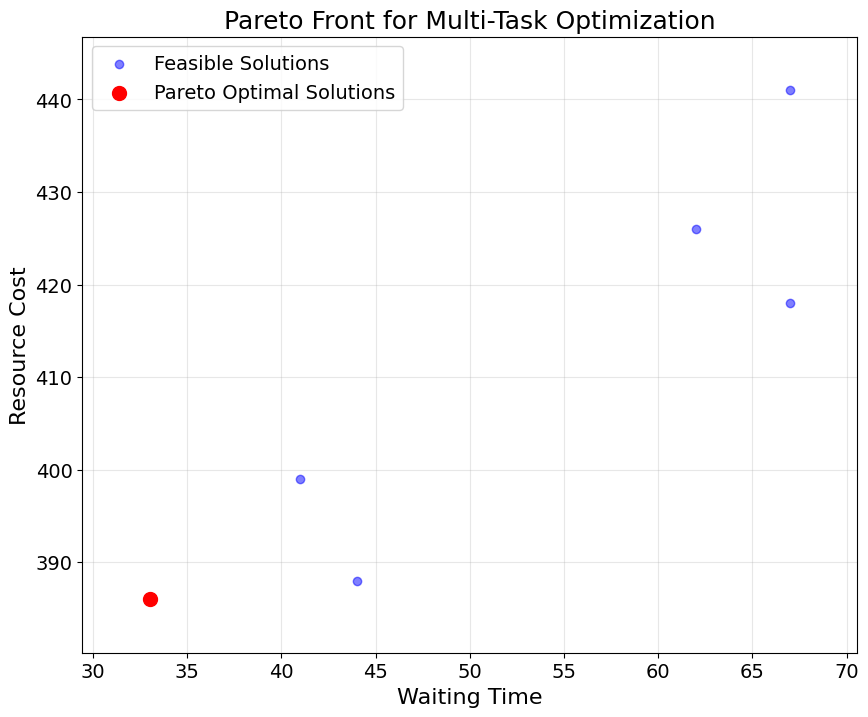
\includegraphics[width=0.8\linewidth, height=8cm]{./images/parato_job6.png}
    \caption{計算できる最大規模数(job数が6)のパレート解}
    \label{fig:fig4}
\end{figure}
\clearpage

\begin{table}[ht]
    \centering
    \vspace{-0.3cm}
    \caption{最大規模数の各巡回における実行可能解と個数および平均値}
    \begin{tabular}{|c|c|c|c|}
        \hline
         巡回 & 個数 & Resource Costの平均値 & Waiting Timeの平均値 \\
        \hline
        第1巡 & 2 & 403 & 55.5 \\
        \hline
        第2巡 & 1 & 426 & 62 \\
        \hline
        第3巡 & 0 & - & - \\
        \hline
        第4巡 & 2 & 420 & 54 \\
        \hline
        第5巡 & 1 & 386 & 33 \\
        \hline
        全体の平均 & 1.5 & 408.8 & 51.1 \\
        \hline
    \end{tabular}
    \label{tab:before_feasible_max}
\end{table}

表\ref{tab:before_feasible_max}と図\ref{fig:fig4}はペトリネット変換前のMRFSSPの計算できる最大規模(job数が6)の時の結果になっている.job数が5の時と比較してパレート解の個数が減少していることから効率的な解を見つけることが困難であることがわかる.また,規模の拡大に伴いそれぞれの目的関数の値の増加も見られる.

\section{考察}
現時点での結果として得られたパレートフロントの形状から,複数の目的関数がトレードオフの関係になっていることが明らかとなった.具体的には,Waiting Timeを短縮するとResource Costが増加し,逆にResource Costを抑制するとWaiting Timeが増加する傾向が確認される.この結果は,どの目的関数を優先するかによって選択される解が異なることを示しており,パレートフロント上の解を選択することで効率的かつ実用的な意思決定を行えると考えられる.実行可能解の個数が少ない原因としては,各パラメータの範囲に対する制限の厳しさが影響している可能性があると考えられる.また,探索回数を100回に限定しているため,解空間の十分な探索が行われず,実行可能解が少なくあった可能性も示唆される.この結果は,パラメータ範囲の設定や探索回数の増加が解空間の拡大および実行可能解の増加に寄与する可能性があると思われる.

さらに,ジョブ数が5から6に増加した場合,Resource Costは約100,Waiting Timeは約3増加することが確認された.Resource Costの増加は,ジョブ数の増加に伴いリソースの割り当てが増加したことに起因すると考えられる.一方,Waiting Timeの増加は,リソースの競合が激化しタスク処理の待機時間が延びたためと推測される.ジョブ数の増加により探索空間が指数関数的に拡大し探索効率が低下することが課題として挙げられる.この課題を克服するためには,解の多様性を維持しつつ探索効率を向上させるアルゴリズムの導入が必要である.特に,大規模問題への適用においては探索空間を効率的に絞り込む手法などの調整が求められる.
